\section{Experiments}
\label{section:exp}
\begin{table*}[t]
\centering
\caption{Comparison of different editing methods. \textbf{Bold} indicates the
best and \uline{underline} the second best; darker colour indicates better
performance within a column.}
\label{tab:method_comparison_wo_kvedit}
\resizebox{\textwidth}{!}{%
\begin{tabular}{l l c c c c c c c c c c c}
\toprule
Method & Base Model & Param. & S.D.$\downarrow$ & PSNR$\uparrow$ & SSIM$\uparrow$ & LPIPS$\downarrow$ & CLIP whole$\uparrow$ & CLIP edited$\uparrow$ & HPSv2$^{\ddag}\uparrow$ & ImgReward$^{\ddag}\uparrow$ & Resolution & Inf. Time$\downarrow$\\
\midrule
Prompt-to-Prompt \cite{prompt2prompt} & Diffusion & 2B
& \AutoCellDown{0.0694}{0.0222}{0.0694}{0}
& \AutoCellUp{17.87}{17.87}{25.33}{0}
& \AutoCellUp{0.7114}{0.7114}{0.8565}{0}
& \AutoCellDown{0.2088}{0.0833}{0.2088}{0}
& \AutoCellUp{0.2501}{0.2280}{0.2642}{0}
& \AutoCellUp{0.2244}{0.2054}{0.2337}{0}
& \AutoCellUp{0.2592}{0.2035}{0.2931}{0}
& \AutoCellUp{-0.0111}{-0.8649}{0.7344}{0}
& 0.5k
& 13.6 \\

Pix2Pix-Zero \cite{pix2pix-zero} & Diffusion & \textasciitilde1B
& \AutoCellDown{0.0617}{0.0222}{0.0694}{0}
& \AutoCellUp{20.44}{17.87}{25.33}{0}
& \AutoCellUp{0.7467}{0.7114}{0.8565}{0}
& \AutoCellDown{0.1722}{0.0833}{0.2088}{0}
& \AutoCellUp{0.2280}{0.2280}{0.2642}{0}
& \AutoCellUp{0.2054}{0.2054}{0.2337}{0}
& \AutoCellUp{0.2338}{0.2035}{0.2931}{0}
& \AutoCellUp{-0.0375}{-0.8649}{0.7344}{0}
& 0.5k
& 17.0 \\

MasaCtrl \cite{masactrl} & Diffusion & \textasciitilde1B
& \AutoCellDown{0.0284}{0.0222}{0.0694}{0}
& \AutoCellUp{22.17}{17.87}{25.33}{0}
& \AutoCellUp{0.7967}{0.7114}{0.8565}{0}
& \AutoCellDown{0.1066}{0.0833}{0.2088}{0}
& \AutoCellUp{0.2396}{0.2280}{0.2642}{0}
& \AutoCellUp{0.2116}{0.2054}{0.2337}{0}
& \AutoCellUp{0.2399}{0.2035}{0.2931}{0}
& \AutoCellUp{-0.1373}{-0.8649}{0.7344}{0}
& 0.5k
& 12.6 \\

PnP \cite{PnP} & Diffusion & \textasciitilde1B
& \AutoCellDown{0.0282}{0.0222}{0.0694}{0}
& \AutoCellUp{22.28}{17.87}{25.33}{0}
& \AutoCellUp{0.7905}{0.7114}{0.8565}{0}
& \AutoCellDown{0.1134}{0.0833}{0.2088}{0}
& \AutoCellUp{0.2541}{0.2280}{0.2642}{0}
& \AutoCellUp{0.2255}{0.2054}{0.2337}{0}
& \AutoCellUp{0.2644}{0.2035}{0.2931}{0}
& \AutoCellUp{0.3242}{-0.8649}{0.7344}{0}
& 0.5k
& 8.0 \\

PnP Inversion \cite{PnP_Inversion} & Diffusion & \textasciitilde1B
& \AutoCellDown{0.0243}{0.0222}{0.0694}{1}
& \AutoCellUp{22.46}{17.87}{25.33}{0}
& \AutoCellUp{0.7968}{0.7114}{0.8565}{0}
& \AutoCellDown{0.1061}{0.0833}{0.2088}{0}
& \AutoCellUp{0.2541}{0.2280}{0.2642}{0}
& \AutoCellUp{0.2262}{0.2054}{0.2337}{0}
& \AutoCellUp{0.2693}{0.2035}{0.2931}{0}
& \AutoCellUp{0.4111}{-0.8649}{0.7344}{0}
& 0.5k
& 8.0 \\

LEDits++ \cite{LEDits++} & Diffusion & \textasciitilde1B
& \AutoCellDown{0.0431}{0.0222}{0.0694}{0}
& \AutoCellUp{19.64}{17.87}{25.33}{0}
& \AutoCellUp{0.7767}{0.7114}{0.8565}{0}
& \AutoCellDown{0.1334}{0.0833}{0.2088}{0}
& \AutoCellUp{0.2642}{0.2280}{0.2642}{0}
& \AutoCellUp{0.2337}{0.2054}{0.2337}{0}
& \AutoCellUp{0.2035}{0.2035}{0.2931}{0}
& \AutoCellUp{-0.8649}{-0.8649}{0.7344}{0}
& 0.5k
& 2.8 \\
\midrule
FlowEdit \cite{Flowedit} & Flow & 12B
& \AutoCellDown{0.0283}{0.0222}{0.0694}{0}
& \AutoCellUp{21.86}{17.87}{25.33}{0}
& \AutoCellUp{0.8368}{0.7114}{0.8565}{0}
& \AutoCellDown{0.1100}{0.0833}{0.2088}{0}
& \AutoCellUp{0.2605}{0.2280}{0.2642}{0}
& \AutoCellUp{0.2281}{0.2054}{0.2337}{0}
& \AutoCellUp{0.2931}{0.2035}{0.2931}{0}
& \AutoCellUp{0.7229}{-0.8649}{0.7344}{0}
& 0.5k
& 6.5 \\

RF-Inversion \cite{RF-inversion} & Flow & 12B
& \AutoCellDown{0.0406}{0.0222}{0.0694}{0}
& \AutoCellUp{20.82}{17.87}{25.33}{0}
& \AutoCellUp{0.7192}{0.7114}{0.8565}{0}
& \AutoCellDown{0.1900}{0.0833}{0.2088}{0}
& \AutoCellUp{0.2520}{0.2280}{0.2642}{0}
& \AutoCellUp{0.2211}{0.2054}{0.2337}{0}
& \AutoCellUp{0.2847}{0.2035}{0.2931}{1}
& \AutoCellUp{0.5484}{-0.8649}{0.7344}{0}
& 1k
& 24.8 \\

ReFlex \cite{ReFlex} & Flow & 12B
& \AutoCellDown{0.0312}{0.0222}{0.0694}{0}
& \AutoCellUp{25.33}{17.87}{25.33}{0}
& \AutoCellUp{0.8436}{0.7114}{0.8565}{1}
& \AutoCellDown{0.0961}{0.0833}{0.2088}{0}
& \AutoCellUp{0.2602}{0.2280}{0.2642}{0}
& \AutoCellUp{0.2266}{0.2054}{0.2337}{0}
& \AutoCellUp{0.2769}{0.2035}{0.2931}{0}
& \AutoCellUp{0.7334}{-0.8649}{0.7344}{1}
& 1k
& 12.4 \\

FireFlow \cite{FireFlow} & Flow & 12B
& \AutoCellDown{0.0222}{0.0222}{0.0694}{0}
& \AutoCellUp{23.80}{17.87}{25.33}{0}
& \AutoCellUp{0.8211}{0.7114}{0.8565}{0}
& \AutoCellDown{0.1168}{0.0833}{0.2088}{0}
& \AutoCellUp{0.2348}{0.2280}{0.2642}{0}
& \AutoCellUp{0.2084}{0.2054}{0.2337}{0}
& \AutoCellUp{0.2551}{0.2035}{0.2931}{0}
& \AutoCellUp{-0.3778}{-0.8649}{0.7344}{0}
& 0.5k
& 2.5 \\
\midrule
AREdit$^\dag$ \cite{AREdit} & VAR & 2B
& \AutoCellDown{0.0305}{0.0222}{0.0694}{0}
& \AutoCellUp{24.19}{17.87}{25.33}{1}
& \AutoCellUp{0.8370}{0.7114}{0.8565}{0}
& \AutoCellDown{0.0870}{0.0833}{0.2088}{1}
& \AutoCellUp{0.2542}{0.2280}{0.2642}{0}
& \AutoCellUp{0.2277}{0.2054}{0.2337}{0}
& --
& --
& 1k
& 2.5 \\
\rowcolor{gray!10}
Ours & VAR & 2B
& \AutoCellDown{0.0316}{0.0222}{0.0694}{0}
& \AutoCellUp{23.44}{17.87}{25.33}{0}
& \AutoCellUp{0.8565}{0.7114}{0.8565}{0}
& \AutoCellDown{0.0833}{0.0833}{0.2088}{0}
& \AutoCellUp{0.2613}{0.2280}{0.2642}{1}
& \AutoCellUp{0.2290}{0.2054}{0.2337}{1}
& \AutoCellUp{0.2785}{0.2035}{0.2931}{0}
& \AutoCellUp{0.7344}{-0.8649}{0.7344}{0}
& 1k
& 2.5 \\
\bottomrule
\end{tabular}%
}
\vspace{1pt}
\raggedright{\footnotesize $^\dag$Results cited from the original paper; no
official implementation has been released, so HPSv2 and ImageReward cannot be
computed for it.\\
$^\ddag$HPSv2 and ImageReward are human-preference metrics we additionally
measure; they are \emph{not} part of the six official PIE-Bench metrics (S.D.,
PSNR, SSIM, LPIPS, CLIP whole, CLIP edited).}
\end{table*}



\subsection{Experimental Settings}

\noindent\textbf{Benchmark.}
We evaluate on PIE-Bench~\cite{PIEBench}, a comprehensive benchmark comprising 700 images (both natural and artificial) across 10 editing categories, including object replacement, addition, removal, attribute modification, and style transfer.

\noindent\textbf{Metrics.}
Following prior work~\cite{PIEBench,AREdit}, we adopt six metrics grouped into two aspects. For \textit{background preservation}, we report Structure Distance~\cite{PIEBench} (S.D.), PSNR, SSIM, and LPIPS~\cite{LPIPS}. For \textit{editing quality}, we report CLIP similarity~\cite{CLIP} on both the whole image (CLIP whole) and the edited region (CLIP edited). We additionally report two preference models, HPSv2 and ImageReward, which we use throughout Sec.~\ref{sec:analysis}. All metrics are computed using the official PIE-Bench evaluation pipeline; generation is performed at 1k resolution while every metric is computed at $512\times512$ under the standard PIE-Bench protocol. Inference time per image is also reported.

Beyond these six official metrics we additionally measure two \textit{human-preference} models, HPS~v2.1~\cite{hpsv2} and ImageReward~\cite{imagereward}. They are not part of the PIE-Bench metric set; we report them because CLIP similarity measures only image--text alignment and is insensitive both to whether the edit was actually carried out and to whether the result agrees with human preference. One convention has to be stated explicitly: every score we report is computed against the \texttt{editing\_prompt} of the PIE-Bench \texttt{mapping\_file.json}, with its bracket annotations removed. This matters for comparability --- scoring the same images against a paraphrase of that prompt shifts ImageReward by as much as $0.33$, enough to invalidate any comparison that mixes the two conventions. Appendix~\ref{app:eval} documents the full protocol.

\noindent\textbf{Baselines.}
We compare with 11 training-free editing methods spanning three architectural families: six diffusion-based --- Prompt-to-Prompt~\cite{prompt2prompt}, Pix2Pix-Zero~\cite{pix2pix-zero}, MasaCtrl~\cite{masactrl}, PnP~\cite{PnP}, PnP Inversion~\cite{PnP_Inversion}, and LEDits++~\cite{LEDits++} --- four flow-based --- FlowEdit~\cite{Flowedit}, RF-Inversion~\cite{RF-inversion}, ReFlex~\cite{ReFlex}, and FireFlow~\cite{FireFlow} --- and one autoregressive method, AREdit~\cite{AREdit}. Baseline results are obtained using officially released code under default settings, except AREdit whose results are cited directly from the original paper as no official implementation has been released.
% TODO(baselines): add the other VAR-based editors (EditInfinity, BitResEdit,
% VARIN) to this list, to Table I, and to Sec. III; add two columns to Table I
% for mask source (external segmentation / hand-drawn / automatic attention) and
% for whether per-image optimization is required.

\noindent\textbf{Implementation details.}
We build upon Infinity~\cite{Infinity} (2B parameters) with BSQ-VAE~\cite{BSQVAE} ($d{=}32$). Generation uses $S{=}13$ scales ($1{\times}1$ to $64{\times}64$), CFG scale 4.0, and temperature $0.5$. Text conditioning uses Flan-T5-XL~\cite{flan-t5}. We set $N{=}2$ anchoring scales. For mask binarization we use the instance-adaptive threshold of Sec.~\ref{sec:threshold} with $h{=}0.50$, $c_{\min}{=}0$, $c_{\max}{=}0.33$, $\kappa_{\min}{=}0$, $\kappa_{\max}{=}0.43$ and $\ell = h - 0.01 = 0.49$; Sec.~\ref{sec:calibration} describes how they are obtained. For IQR filtering, we discard transformer blocks whose attention deviation from the cross-block mean exceeds the IQR fence (Sec.~\ref{sec:mask_construction}), using blocks 2--31 of the 32-block model (blocks 0--1 are excluded as they consistently exhibit the global attention effect described in Sec.~\ref{sec:mask_construction}). All experiments run on a single NVIDIA RTX 5090 GPU with ${\sim}$2.5\,s inference per image.
%% Verified 2026-08-13 against the run behind the main table:
%% pie_edit_rewrite_minimal_m15_h0.50_k0-0.43_cum0_N2 (method 15, h=0.50,
%% cv[0,0.33], kappa[0,0.43], l=0.49, cum0, N=2, minimal rewrite, seed 1, n=700).
%% Measured runtime tau median 0.537 over all scales.

\subsection{Comparison with State-of-the-Art Methods}

\noindent\textbf{Quantitative results.}
Table~\ref{tab:method_comparison_wo_kvedit} summarizes the comparison. Our
method attains the best SSIM ($0.8565$) and LPIPS ($0.0833$) of any method
compared, and the second-best CLIP whole ($0.2613$) and CLIP edited ($0.2290$),
showing strong background preservation together with competitive edit quality
from a 2B backbone --- one sixth of the parameters of every flow-based baseline.
We are not best on Structure Distance or PSNR, and this reflects the choice of
operating point: as Sec.~\ref{sec:frontier} shows, background preservation and
edit strength trade off along a continuous frontier, and we select a point that
balances the two.

\noindent\textbf{Human-preference metrics.}
On the two additional preference metrics our ImageReward is $0.7344$, essentially
identical to the closest baseline ReFlex ($0.7334$); the gap of $0.001$ is far
below the full-benchmark run-to-run spread (about $\pm 0.02$,
Sec.~\ref{sec:analysis}), so the two should be read as \textit{level} rather
than as a lead. The substantive conclusion on ImageReward is that we are on par
with two 12B flow-based models (ReFlex, and FlowEdit at $0.7229$) with one sixth
of their parameters. On HPSv2 we reach $0.2785$, third behind FlowEdit
($0.2931$) and RF-Inversion ($0.2847$). No official implementation of AREdit has
been released, so we cannot obtain its outputs and cannot compute either metric
for it.

\textit{vs.\ diffusion-based methods.}
Compared to the best diffusion-based method PnP Inversion, we improve SSIM by $7.5\%$ and LPIPS by $21.5\%$ while achieving higher CLIP scores on both whole-image and edited-region metrics.

\textit{vs.\ flow-based methods.}
Against the strongest flow-based competitor ReFlex, we attain better SSIM and
LPIPS despite the $6\times$ parameter gap, though ReFlex achieves higher PSNR.

\textit{vs.\ AREdit.}
AREdit~\cite{AREdit} is the closest comparison: a training-free editor on the same 2B VAR backbone. We are better on SSIM, LPIPS and both CLIP metrics, while AREdit is slightly ahead on Structure Distance and PSNR. The more consequential difference is where the mask comes from: AREdit requires the user to supply a threshold per editing category, whereas our masks are derived entirely from the model's own cross-attention with no per-category tuning --- which is precisely the advantage of attention-driven mask construction over cached token statistics.
% TODO(optional): if Table I gains a preservation-oriented row, quote it here.
% A higher-h operating point under this formulation reaches PSNR/S.D. comparable
% to or better than AREdit; that row must come from a direct run under the SAME
% configuration as the rest of Table I before it can be quoted.

We report inference time for reference, but note that methods operate at different generation resolutions; all metrics are nevertheless computed at the common $512\times512$ evaluation resolution.

\begin{figure*}[!t]
    \centering
    \includegraphics[width=\textwidth]{imgs/qualitative.png}
    \caption{Qualitative comparison with FireFlow, FlowEdit, ReFlex, RF-Inversion, LEDits++, MasaCtrl, PnP, and PnP-Inversion across diverse editing types: attribute replacement (smoke$\to$fire), pose change (sitting$\to$standing), object addition (+flowers), and style transfer (watercolor$\to$anime). Notably, the second row shows that our method correctly transforms the bear's pose from sitting to standing while preserving both the background and the bear's visual identity. More results are provided in the appendix.}
    \label{fig:qualitative}
\end{figure*}

\noindent\textbf{Qualitative results.}
Fig.~\ref{fig:qualitative} presents representative visual comparisons. Diffusion-based methods often suffer from structural drift or incomplete edits due to inversion errors: P2P and Pix2Pix-Zero alter the global layout, while MasaCtrl preserves structure but produces blurry edited regions. Among flow-based methods, ReFlex achieves the best preservation but occasionally misses fine-grained edit details. In contrast, our method produces clean, precisely localized edits while faithfully preserving the background, benefiting from explicit attention-driven masking and discrete token replacement.

\subsection{Attention Masking vs.\ Scale-Level Replacement}
\label{sec:ablation_mask}

The most basic alternative to a spatial mask is no spatial mask at all: share the first $N$ scales with the source by full replacement and let every later scale generate freely under $P_t$. We denote this variant Scale-$N$ and vary $N \in \{1, 2, 4, 6\}$.

%% Convention: best in bold.
\begin{table}[t]
\caption{Ablation on attention-based masking. \emph{Scale-$N$}: the first $N$
scales are replaced with source tokens and no attention mask is applied at any
later scale. \emph{Attn Mask}: the full three-phase pipeline. S.D.\ is Structure
Distance. \textbf{Bold} is the best.}
\label{tab:ablation_mask}
\centering
\small
\resizebox{\linewidth}{!}{%
\begin{tabular}{l|cccc|cc}
\toprule
Config & S.D.$\downarrow$ & PSNR$\uparrow$ & SSIM$\uparrow$ & LPIPS$\downarrow$ & CLIPw$\uparrow$ & CLIPe$\uparrow$ \\
\midrule
Scale-1 & 0.0843 & 12.25 & 0.4330 & 0.3930 & 0.2439 & 0.2210 \\
Scale-2 & 0.0807 & 12.56 & 0.4450 & 0.3810 & 0.2427 & 0.2199 \\
Scale-4 & 0.0611 & 14.08 & 0.4960 & 0.3190 & 0.2121 & 0.1946 \\
Scale-6 & 0.0424 & 15.66 & 0.5530 & 0.2560 & 0.2001 & 0.1822 \\
\midrule
Attn Mask (Ours) & \textbf{0.0316} & \textbf{23.44} & \textbf{0.8565} & \textbf{0.0833} & \textbf{0.2613} & \textbf{0.2290} \\
\bottomrule
\end{tabular}}
\end{table}

\begin{figure}[t]
    \centering
    \begin{subfigure}[t]{1\linewidth}
        \centering
        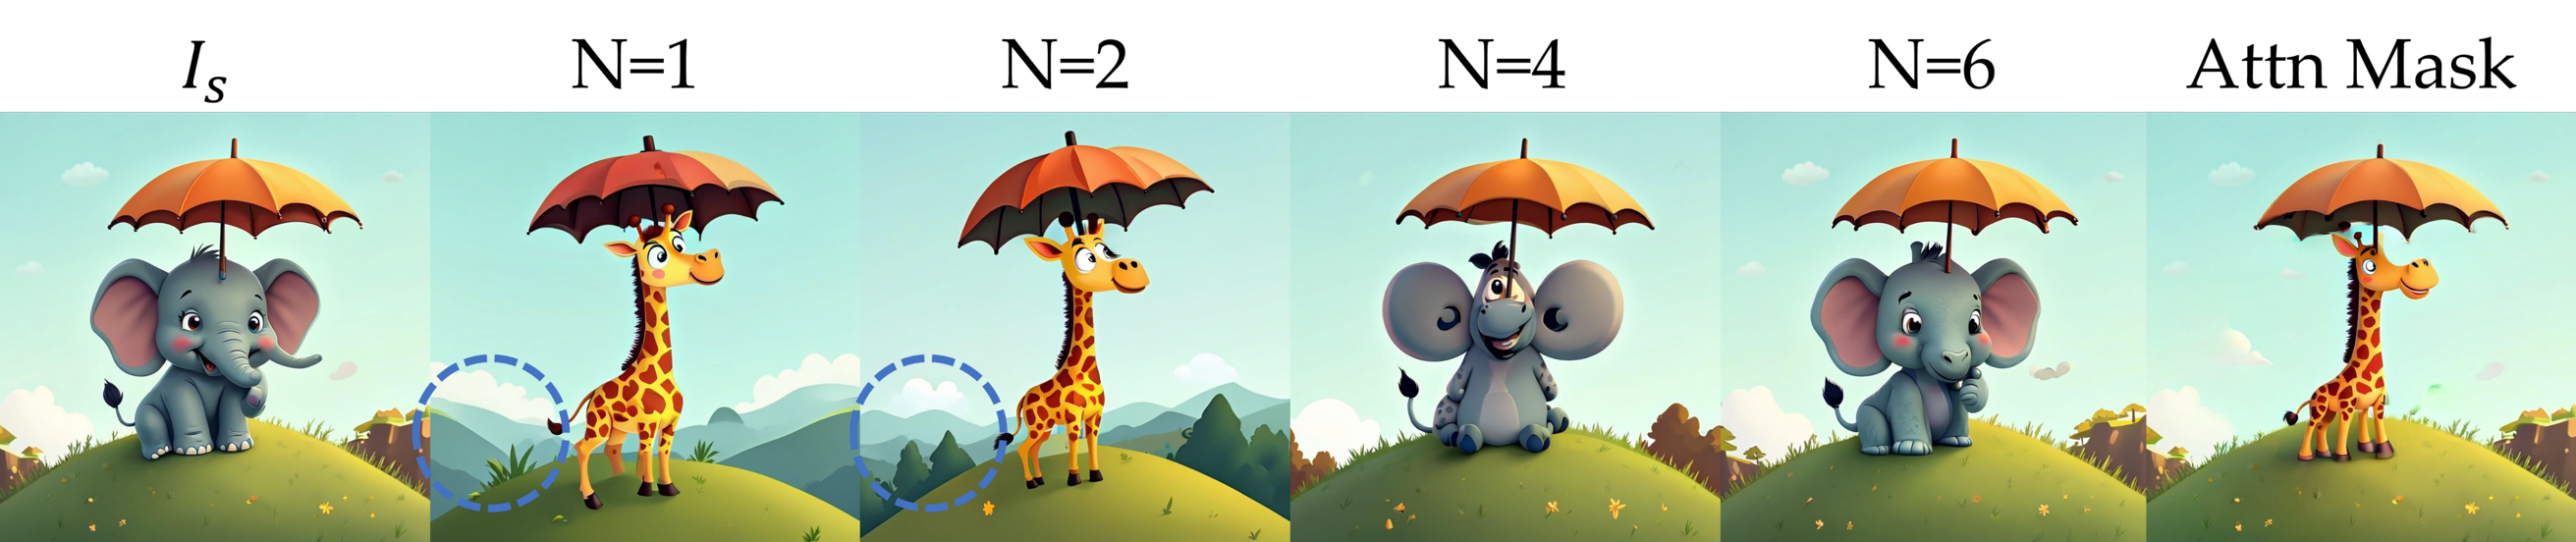
\includegraphics[width=\linewidth]{imgs/shape_diff.png}
        \caption{Scale-$N$ replacement: few shared scales allow editing but lose the background; many shared scales preserve the background but lock the subject. Our attention-mask approach achieves both precise editing and faithful preservation.}
        \label{fig:shape_diff_a}
    \end{subfigure}
    \hfill
    \begin{subfigure}[t]{1\linewidth}
        \centering
        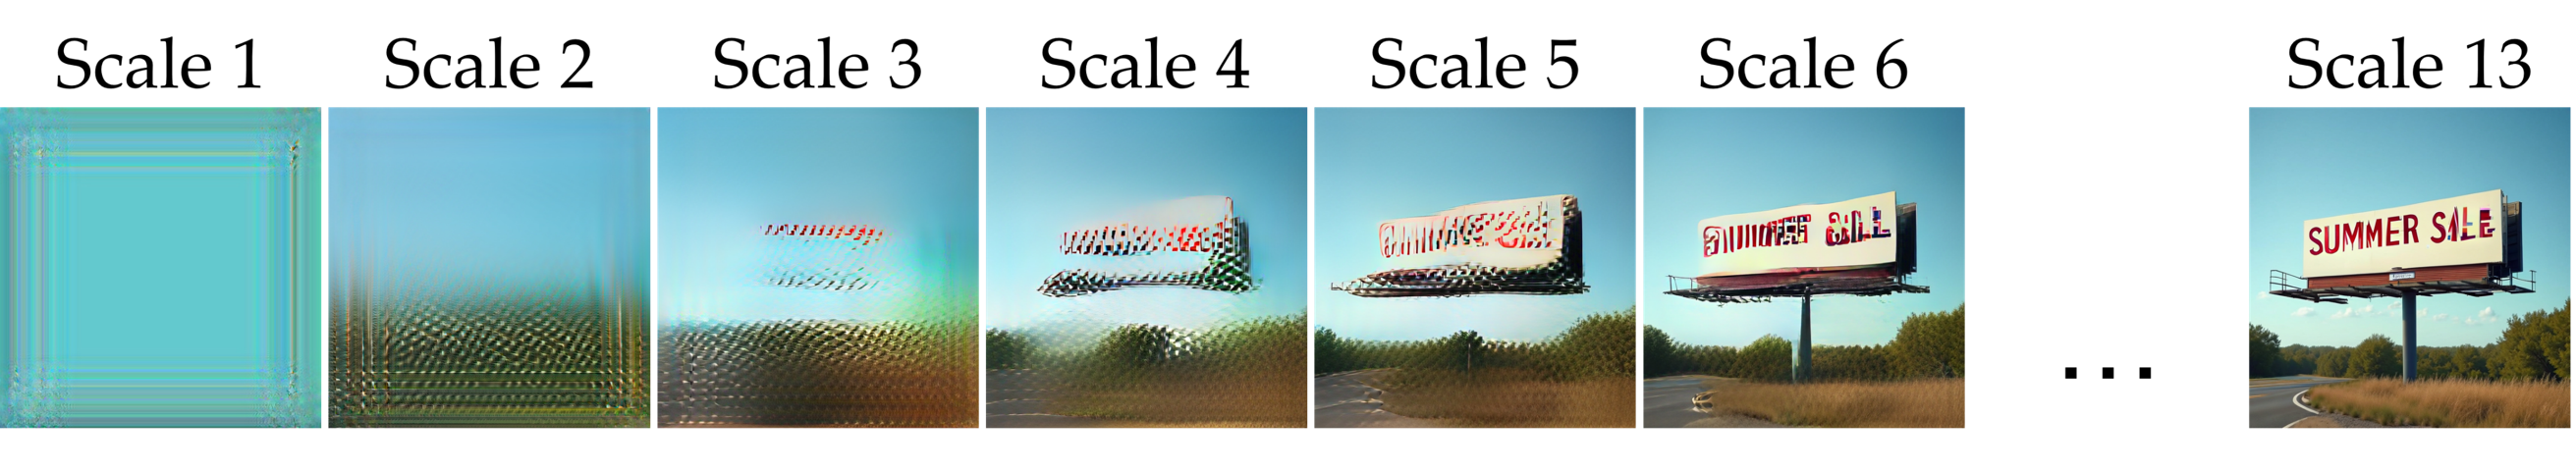
\includegraphics[width=\linewidth]{imgs/coarse2fine.png}
        \caption{VAR's coarse-to-fine generation: early scales ($k \leq 4$) determine global layout; later scales refine texture. Fixed-scale replacement thus cannot accommodate shape-changing edits.}
        \label{fig:shape_diff_b}
    \end{subfigure}
    \caption{Analysis of scale-level replacement vs.\ attention-based masking. (a) Comparison across configurations on an elephant $\to$ giraffe edit. (b) VAR's coarse-to-fine generation: early scales commit to global layout, limiting the effectiveness of fixed-scale replacement strategies.}
    \label{fig:shape_diff}
\end{figure}

As shown in Table~\ref{tab:ablation_mask}, increasing the number of shared scales progressively improves preservation, but the gains saturate: even at $N{=}6$ --- nearly half of the 13 scales --- SSIM reaches only $0.553$, because every scale beyond $N$ generates with no reference to the source. Per-token spatial guidance at every scale improves SSIM by 55\% and LPIPS by 67.5\% over the best Scale-$N$ variant.

Fig.~\ref{fig:shape_diff} explains why the saturation is structural rather than a matter of choosing $N$ better. Fig.~\ref{fig:shape_diff_a} shows the two failure modes at the ends of the range: few shared scales permit the edit but destroy the background, while many shared scales preserve the background and simultaneously lock the subject, since the global layout is already committed. Fig.~\ref{fig:shape_diff_b} shows the underlying cause --- VAR fixes the global arrangement within the first few scales and spends the remainder on texture --- so a shape-changing edit must modify early tokens, which uniform scale-level replacement cannot do selectively. Attention masking resolves the tension by replacing only background positions at every scale, which is what makes precise editing and faithful preservation simultaneously attainable. The residual cost of the coarse anchoring that remains is analyzed in Sec.~\ref{sec:limitations}.

\subsection{Phase 2}
\label{sec:ablation_phase2}

Phase~2 performs a second generation pass under the target prompt in order to
extract the target focus mask $M_{k,t}^{\mathrm{f}}$ before any token is replaced
(Sec.~\ref{sec:pipeline}). We compare the full three-phase pipeline against a
variant that skips Phase~2 entirely.

%% Translated from NTUST_Thesis_Kai/tabs/ablationPhase2.tex.
%% Simple two-arm ablation: the full three-phase pipeline versus the same
%% pipeline with Phase 2 skipped entirely.
%% Convention: best in bold (two rows only, so no second-best mark).
\begin{table}[t]
\centering
\caption{Ablation of Phase~2. \textbf{Bold} is the best.}
\label{tab:ablation_phase2}
\small
\resizebox{\linewidth}{!}{%
\begin{tabular}{l|cccc|cc}
\toprule
Method & S.D.$\downarrow$ & PSNR$\uparrow$ & SSIM$\uparrow$ & LPIPS$\downarrow$ & CLIPw$\uparrow$ & CLIPe$\uparrow$ \\
\midrule
With Phase 2 & \textbf{0.0316} & \textbf{23.44} & \textbf{0.8565} & \textbf{0.0833} & \textbf{0.2613} & \textbf{0.2290} \\
W/O Phase 2  & 0.0518 & 17.02 & 0.6228 & 0.2047 & 0.2522 & 0.2212 \\
\bottomrule
\end{tabular}%
}
\end{table}


As shown in Table~\ref{tab:ablation_phase2}, Phase~2 is the single largest
contribution of any component: PSNR improves by $37.7\%$, SSIM by $37.5\%$,
LPIPS drops by $59.3\%$ and Structure Distance by $39.0\%$, with the CLIP scores
also rising by $3.5$--$3.6\%$. These results confirm that a source-side mask alone
cannot delineate the edit boundary accurately --- least of all when the target
introduces spatial content that does not exist in the source. The dual-stream
mask construction of Phases~1--2 is therefore indispensable for achieving precise
edits without background drift.

\subsection{IQR Filtering}
\label{sec:ablation_iqr}

Not all transformer blocks produce equally informative attention maps. As described in Sec.~\ref{sec:mask_construction}, we measure each block's deviation from the cross-block mean and discard outlier blocks whose deviation exceeds the IQR fence. We compare our full model against naively averaging all blocks.

%% Split out from the old tabs/ablationThreshold.tex: only the IQR part remains
%% here, since the "adaptive vs fixed percentile" comparison belonged to the
%% rank-based formulation and is superseded by Sec. V-B / V-C.
\begin{table}[t]
\centering
\caption{Ablation on IQR block filtering. Removing the filter and averaging all
blocks lets positional-bias-dominated attention corrupt the mask. Both rows are
measured under one common configuration held fixed across the ablation, which is
not the operating point reported in
Table~\ref{tab:method_comparison_wo_kvedit}; the comparison between rows is
unaffected. Nothing is marked.}
\label{tab:ablation_iqr}
\small
\resizebox{\linewidth}{!}{%
\begin{tabular}{l|cccc|cc}
\toprule
Method & S.D.$\downarrow$ & PSNR$\uparrow$ & SSIM$\uparrow$ & LPIPS$\downarrow$ & CLIPw$\uparrow$ & CLIPe$\uparrow$ \\
\midrule
\rowcolor{gray!12}
With IQR & 0.0316 & 23.44 & 0.8565 & 0.0833 & 0.2613 & 0.2290 \\
W/O IQR   & 0.0328 & 20.56 & 0.7872 & 0.1285 & 0.2550 & 0.2260 \\
\bottomrule
\end{tabular}%
}
\end{table}

% \begin{figure}[t]
%     \centering
%     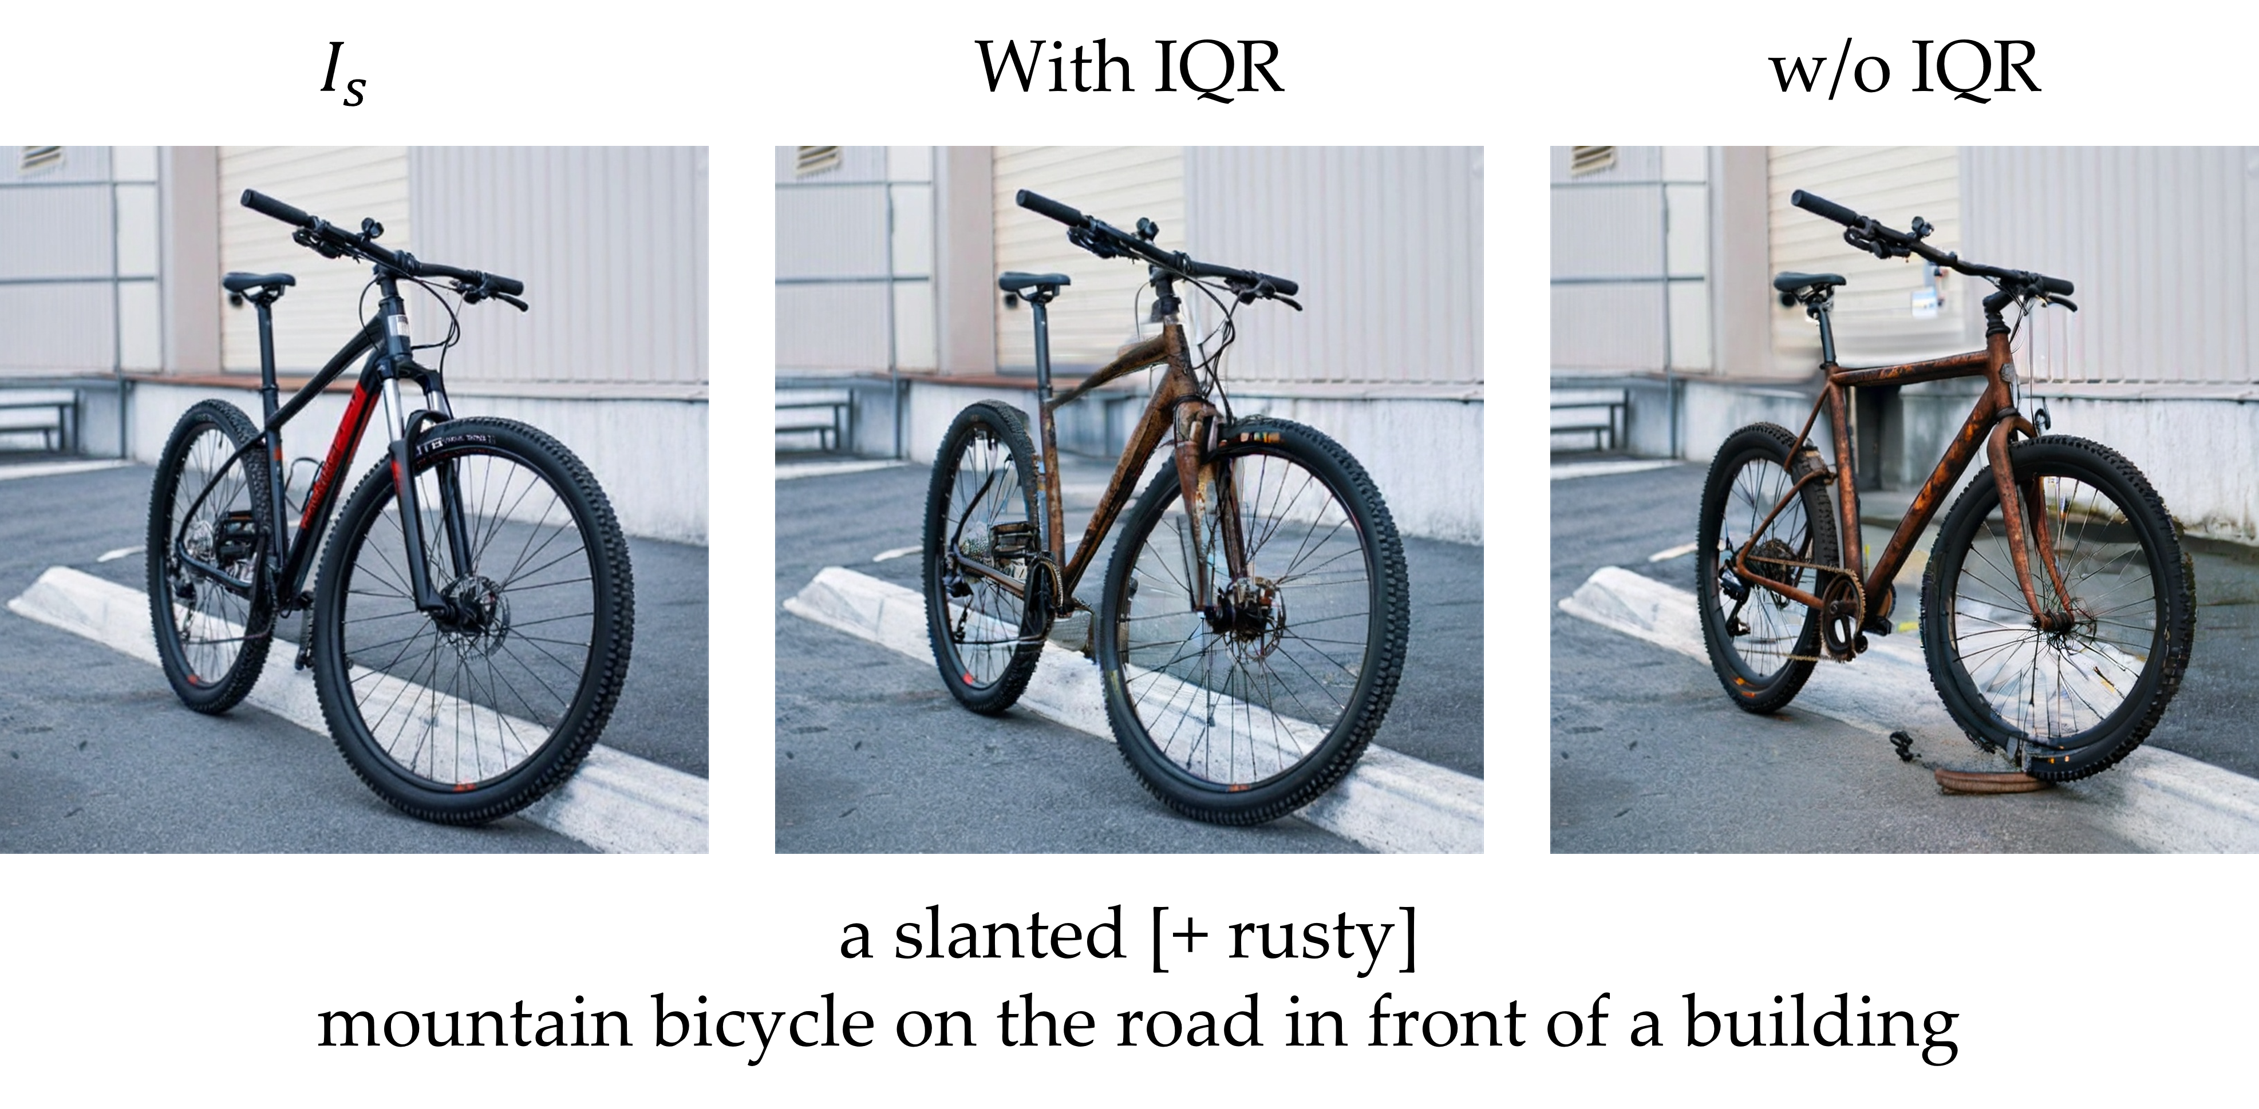
\includegraphics[width=\linewidth]{imgs/ablationIQR.png}
%     \caption{Effect of IQR filtering on editing quality. $I_s$ denotes the source image. With IQR filtering, the generated mask accurately captures the editing region, preserving the overall structure of the bicycle. Without IQR filtering, the bicycle structure is severely distorted, demonstrating that IQR-based block selection is critical for producing reliable attention masks.}
%     \label{fig:ablationIQR}
% \end{figure}
\begin{figure}[t]
    \centering
    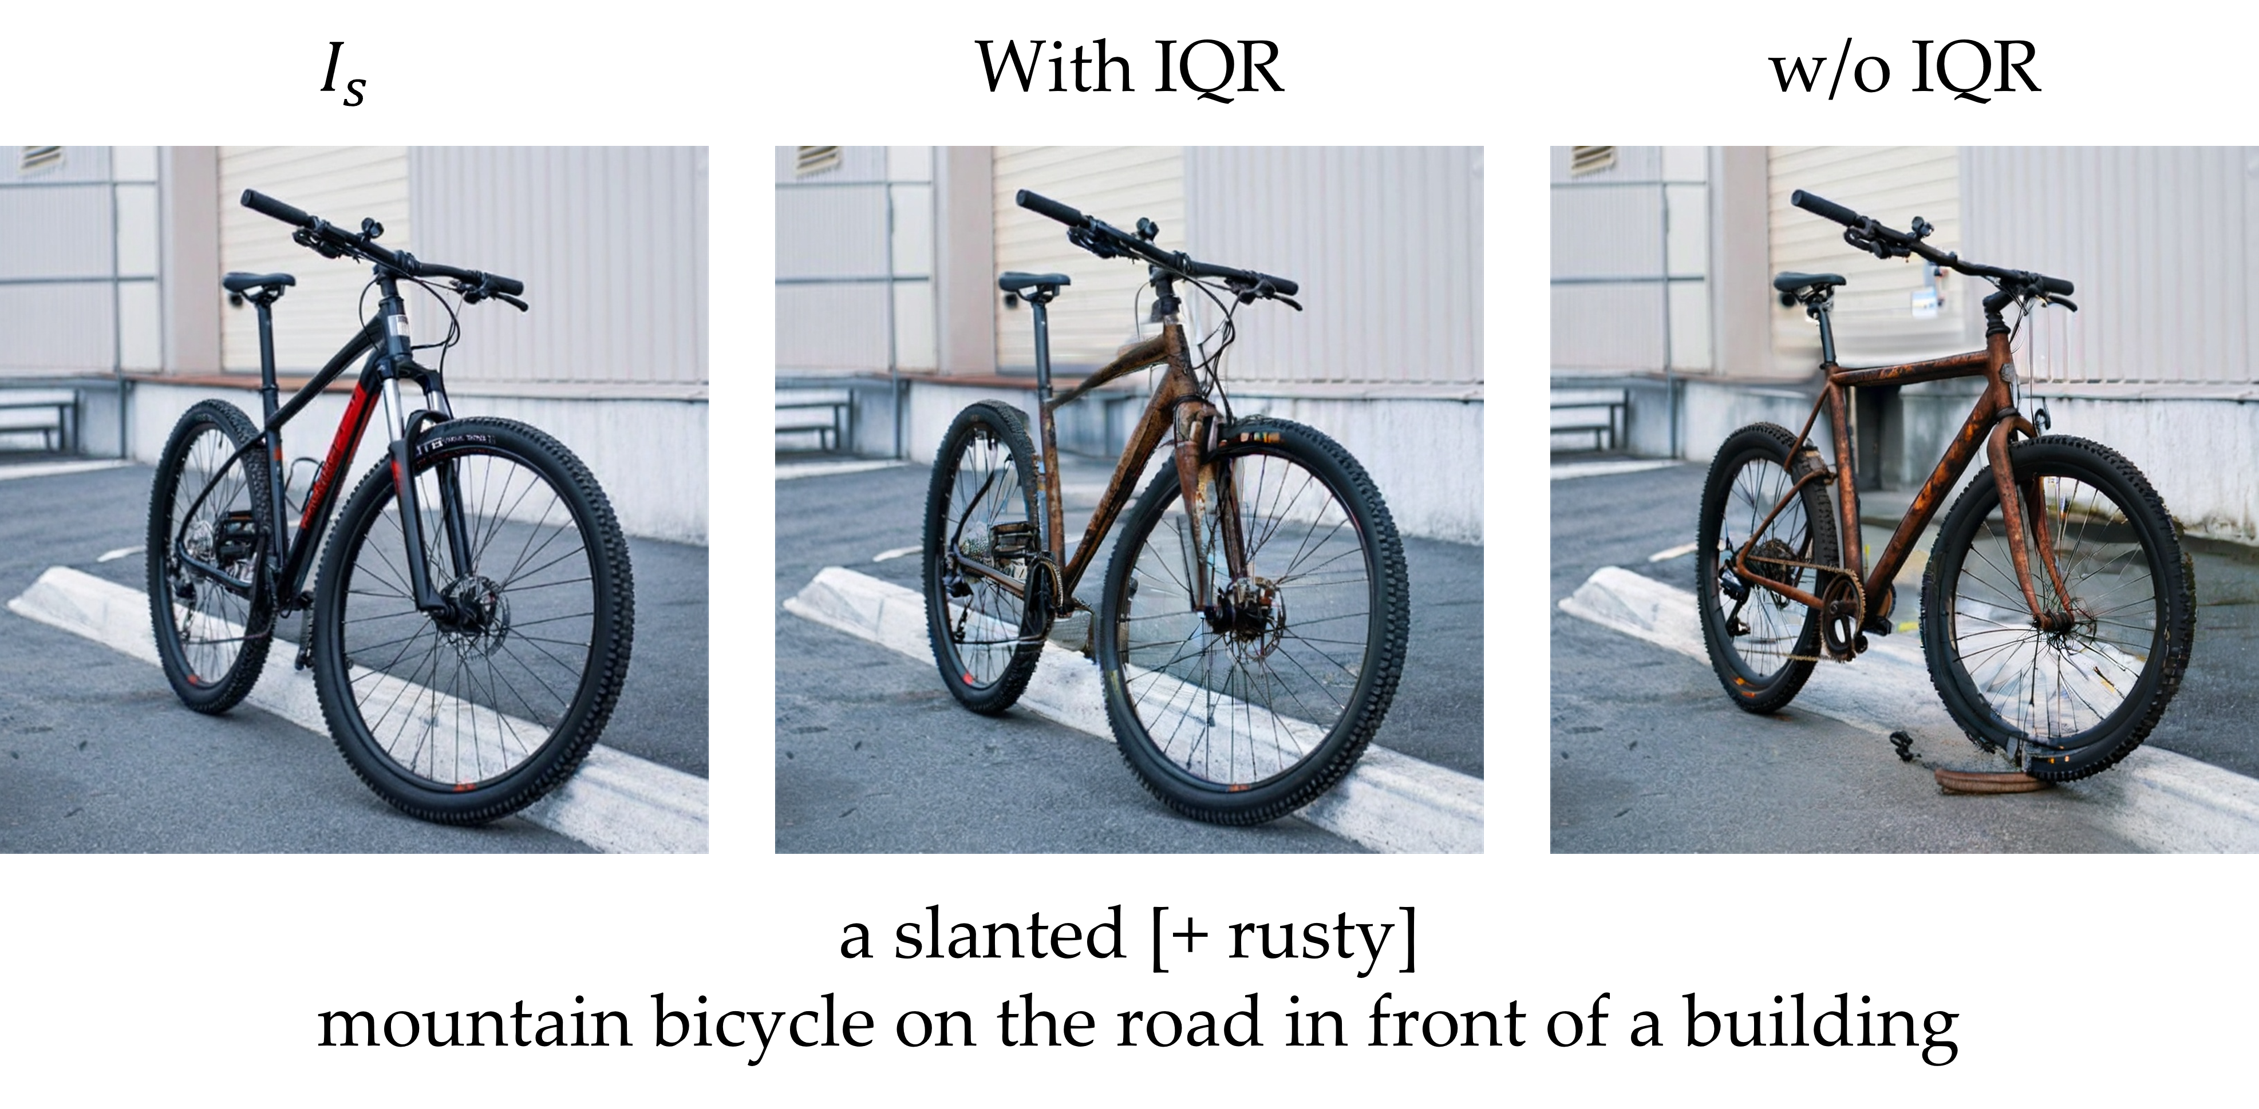
\includegraphics[width=\linewidth]{imgs/ablationIQR.png}
    \caption{Effect of IQR filtering. With filtering, the mask accurately captures the editing region and preserves the bicycle structure. Without it, the structure is severely distorted.}
    \label{fig:ablationIQR}
\end{figure}

As shown in Table~\ref{tab:ablation_iqr}, IQR filtering yields substantial improvements: PSNR increases by 14.0\% and SSIM by 8.8\%, while LPIPS drops by 35.2\%, confirming that filtered masks avoid corrupting non-target regions. Structure Distance also improves ($0.0328 \to 0.0316$), showing that cleaner masks reduce unintended structural changes. Fig.~\ref{fig:ablationIQR} illustrates the effect: without filtering, noisy attention from uninformative blocks produces imprecise masks that distort the bicycle structure; with IQR filtering, the mask cleanly delineates the target.
